% ============================================================================
%  An analytic origin for the provenance bias in radial migration
%  MNRAS pre-print
% ============================================================================
\documentclass[fleqn,usenatbib]{mnras}

\usepackage{graphicx}
\usepackage{amsmath}
\usepackage{amssymb}
\usepackage{txfonts}

\newcommand{\Jz}{J_z}
\newcommand{\Lz}{L_z}
\newcommand{\JR}{J_R}
\newcommand{\hZ}{h_Z}
\newcommand{\sigz}{\sigma_z}
\newcommand{\sigR}{\sigma_R}
\newcommand{\Lsun}{L_\odot}
\newcommand{\kpc}{\,\mathrm{kpc}}

\title[An analytic origin for the provenance bias]{An analytic origin for the
provenance bias in radial migration, and the spiral $\JR$--$\hZ$ relation}

\author[C. Vera-Ciro]{Carlos Vera-Ciro$^{1}$\thanks{E-mail: caverac@gmail.com}\\
$^{1}$Independent Researcher}

\date{Draft. Received YYY; in original form ZZZ}
\pubyear{2026}

\begin{document}
\label{firstpage}
\maketitle

\begin{abstract}
Radial migration in disc galaxies is observed in $N$-body simulations to act
preferentially on stars with small vertical excursions -- the ``provenance
bias'' \citep{VeraCiro2016imprint,Mikkola2020}. The effect is established only
qualitatively (cold stars spend more time near the mid-plane and couple more
readily to the plane-concentrated spiral) and lacks a first-principles
description. We supply one. The coupling of a star to a spiral of radial
wavenumber $k$ is set by the angle-average over its vertical orbit of the
spiral potential's $e^{-k|z|}$ fall-off above the plane -- a \emph{vertical form
factor} $F(\Jz,k)=\langle e^{-k|z|}\rangle$, which equals unity for a mid-plane
orbit and decreases monotonically with vertical action. Inserting $F$ into the
\citet{DanielWyse2015,DanielWyse2018} corotation-capture criterion yields the
provenance bias analytically: with a single physical spiral strength
$s=\sigR^2/|\Phi_s|\approx0.9$ the model reproduces the measured ${\sim}20$ per
cent vertical cooling of migrators at the Milky-Way thickness $\alpha\equiv k\hZ
\approx0.84$, and predicts its dependence on disc thickness and spiral strength
in agreement with the simulations. Because $F$ depends on $k$ and $\hZ$ only
through $\alpha$, the same object links the bias to the empirical spiral-arm
$\JR^{\max}$--$\hZ$ relation \citep{Palicio2024}; the structural slope
$a=c_{\max}(\pi G\Sigma/\kappa)(\sigR/\sigz)^2$ reproduces the measured
$3.7\times10^{-2}\,\Lsun/\kpc$, and is predicted to flatten with population age
as $\mathrm{age}^{2(\beta_R-\beta_z)}$, halving from $1$ to $8\,$Gyr for
literature age--velocity-dispersion exponents -- a falsifiable test with
mono-age samples.
\end{abstract}

\begin{keywords}
Galaxy: disc -- Galaxy: kinematics and dynamics -- galaxies: spiral
\end{keywords}

% ---------------------------------------------------------------------------
\section{Introduction}
\label{sec:intro}

Transient, recurrent spiral arms \citep{DOnghia2013} churn stellar angular
momentum at the corotation resonance, moving stars radially with little heating
\citep{SellwoodBinney2002}. A robust but unexplained feature of this
process is its \emph{vertical selectivity}: in $N$-body discs the stars that
migrate are preferentially those on nearly circular orbits confined to the
plane. \citet{VeraCiro2016imprint} named this the ``provenance bias'' and showed
that it -- rather than vertical heating -- sets the vertical structure of
migrators, with migrating stars some $20$ per cent cooler in $\sigz$ than the
parent population. \citet{Mikkola2020} confirmed that the importance of
migration at large vertical action depends on the spiral strength. Both works
state the mechanism only qualitatively -- cold stars spend more time near the
mid-plane and couple more readily to the spiral -- and \citet{Mikkola2020}
explicitly flag an analytic description as future work.

Independently, \citet{Palicio2024} report a linear relation, found across
simulated spiral galaxies and satisfied by the Milky Way, between the maximum
radial action of spiral-arm stars and the disc vertical scale $\hZ$ -- which they
measure as an exponential vertical scale-length --
$\JR^{\max}=a\,\hZ+b$ with $a\approx3.7\times10^{-2}\,\Lsun/\kpc$
(see also \citealt{Jia2024}); the slope is not derived from first principles.

This Letter provides the missing analytic glue. \citet{DanielWyse2015,
DanielWyse2018} already derived an analytic corotation-capture criterion in
which the captured fraction declines with radial random energy as
$\exp(-\sigR^2/|\Phi_s|)$ -- low-dispersion stars migrate preferentially -- but
their criterion is strictly in-plane. We extend it to the third dimension with a
vertical form factor (Section~\ref{sec:formfactor}), recover the provenance bias
and its trends (Section~\ref{sec:bias}), and tie the same object to the
$\JR^{\max}$--$\hZ$ slope and its age dependence (Section~\ref{sec:slope}).

% ---------------------------------------------------------------------------
\section{The vertical form factor}
\label{sec:formfactor}

A razor-thin spiral perturbation of radial wavenumber $k$ has a potential that
satisfies Laplace's equation above the disc and therefore decays as $e^{-k|z|}$
\citep{BinneyTremaine2008}. A star executing a vertical oscillation
$z(\theta_z;\Jz)$ samples the spiral through the angle-average of that decay,
%
\begin{equation}
  F(\Jz,k) \;=\; \big\langle e^{-k|z(\theta_z,\Jz)|}\big\rangle_{\theta_z}
  \;=\; \frac{2}{\pi}\int_0^{z_m} e^{-kz}\,\frac{\nu_z}{|v_z|}\,\mathrm{d}z,
  \label{eq:formfactor}
\end{equation}
%
with $z_m$ the turning point, $\nu_z$ the vertical frequency and
$v_z=\sqrt{2[E-\Phi(z)]}$. We evaluate \eqref{eq:formfactor} on the
self-consistent isothermal sheet \citep{Spitzer1942}, $\Phi(z)=2\ln\cosh z$ in
units $G=\sigz=z_0=1$, for which the only parameter is the dimensionless
thickness $\alpha\equiv kz_0$. By construction $F(0,k)=1$ -- a mid-plane orbit
feels the full in-plane amplitude -- and $F$ decreases monotonically with
vertical action (Fig.~\ref{fig:formfactor}). This is the quantitative content of
``cold stars couple more readily'': $F$ is precisely the time the orbit spends
near the plane, weighted by the spiral's reach.

For the Milky Way a radial wavelength $\lambda_R\sim3\kpc$
($k=2\pi/\lambda_R\sim2\kpc^{-1}$) and $z_0\sim0.4\kpc$ give $\alpha\sim0.84$ --
of order unity, which is why the bias is an order-$20$ per cent effect rather
than negligible.

The quadrature~\eqref{eq:formfactor} is confirmed by an independent route:
integrating the vertical orbit with the \textsc{galpy} integrator
\citep{Bovy2015} in its isothermal-disc potential and time-averaging $e^{-k|z|}$
over a whole number of vertical periods reproduces $F$ to better than
$2\times10^{-4}$ across the relevant range (Fig.~\ref{fig:validation}).

\begin{figure}
  
\includegraphics[width=\columnwidth]{form-factor.pdf}
  \caption{The vertical form factor $F(\Jz,k)=\langle e^{-k|z|}\rangle$,
  equation~\eqref{eq:formfactor}, versus vertical action for three spiral
  wavenumbers $\alpha=kz_0$. $F\to1$ for mid-plane orbits and falls monotonically
  with $\Jz$: vertically hot stars couple weakly to the spiral. The suppression
  steepens with $\alpha$.}
  \label{fig:formfactor}
\end{figure}

\begin{figure}
  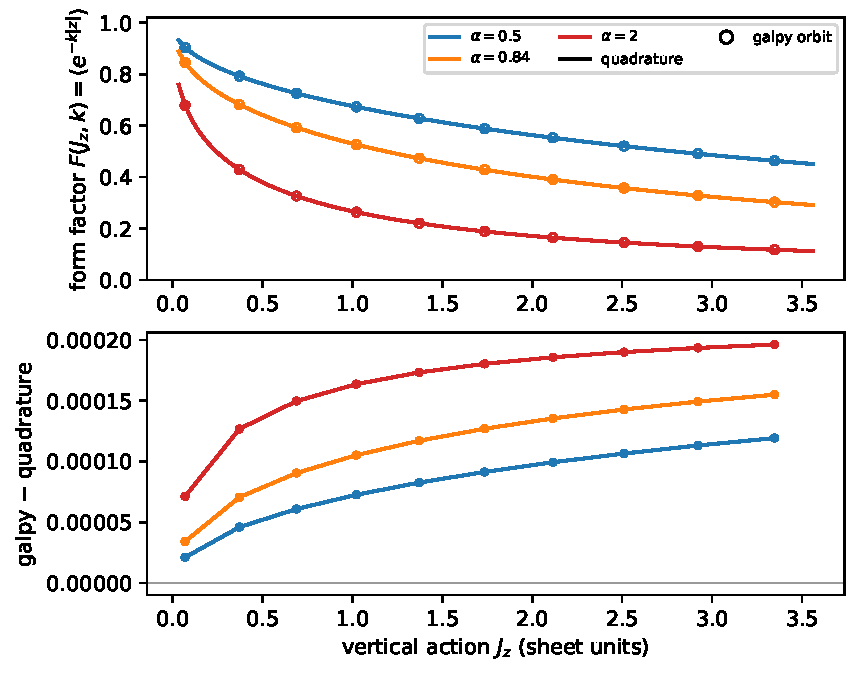
\includegraphics[width=\columnwidth]{form-factor-validation.pdf}
  \caption{Independent validation of the vertical form
  factor~\eqref{eq:formfactor}. The scipy quadrature (curves) and the
  \textsc{galpy} orbit-integrated time-average (markers) agree across vertical
  action for three disc thicknesses $\alpha$; the residual (lower panel) stays
  below $2\times10^{-4}$.}
  \label{fig:validation}
\end{figure}

% ---------------------------------------------------------------------------
\section{The provenance bias}
\label{sec:bias}

\citet{DanielWyse2015,DanielWyse2018} show the corotation-capture fraction of an
in-plane population scales as $\exp(-\sigR^2/|\Phi_s|)$. Reducing the felt well
depth by the vertical form factor, $|\Phi_s|\to|\Phi_s|F(\Jz,k)$, gives the
migration weight of a star of vertical energy $E$,
%
\begin{equation}
  W(\Jz) \;=\; \exp\!\Big[-s\big(1/F(\Jz,k)-1\big)\Big], \qquad
  s \equiv \frac{\sigR^2}{|\Phi_s|},
  \label{eq:weight}
\end{equation}
%
normalised to unity at $F=1$. The single new parameter $s$ is the spiral
strength; $s\sim1$ is the \citet{DanielWyse2015} efficient-capture regime, and
$|\Phi_s|\sim1$--$3$ per cent of $v_c^2$ gives $s\sim0.8$--$2$. Reweighting the
equilibrium vertical distribution $\mathrm{d}N/\mathrm{d}E\propto e^{-E}/\nu_z$
by $W$ yields the migrator dispersion ratio $\sigz^{\rm mig}/\sigz^{\rm all}$.

At the Milky-Way thickness $\alpha=0.84$ the measured $20$ per cent cooling
($\sigz^{\rm mig}/\sigz^{\rm all}\approx0.80$) is reproduced by $s=0.90$ -- well
inside the physical range, with no further freedom. The model predicts a
two-parameter trend (Fig.~\ref{fig:bias}): the bias \emph{weakens} as the spiral
strengthens (small $s$), matching \citet{Mikkola2020} and the morphology
independence of \citet{VeraCiro2016imprint}, and \emph{strengthens} with disc
thickness $\alpha$. A zero-free-parameter test is available: predicting the
relative bias of disc models of different $\alpha$ and $s$ once those are
measured.

\begin{figure}
  
\includegraphics[width=\columnwidth]{provenance-bias.pdf}
  \caption{Predicted migrator vertical cooling
  $1-\sigz^{\rm mig}/\sigz^{\rm all}$ versus disc thickness $\alpha=k\hZ$ at the
  spiral strength $s=0.90$ fixed by the Milky-Way anchor (star;
  \citealt{VeraCiro2016imprint}). The bias is an order-$20$ per cent effect at
  the Galactic $\alpha$ and strengthens for thicker discs.}
  \label{fig:bias}
\end{figure}

% ---------------------------------------------------------------------------
\section{The $\JR^{\max}$--$\hZ$ relation and its age-running}
\label{sec:slope}

The same form factor links the bias to the \citet{Palicio2024} relation.
Combining the isothermal-sheet scale height $\hZ=\sigz^2/(\pi G\Sigma)$ with the
epicyclic action $\JR^{\max}=c_{\max}\sigR^2/\kappa$ gives the slope as the
squared radial-to-vertical heating-anisotropy ratio,
%
\begin{equation}
  a \;=\; \frac{\JR^{\max}}{\hZ}
    \;=\; c_{\max}\,\frac{\pi G\Sigma}{\kappa}\left(\frac{\sigR}{\sigz}\right)^2 .
  \label{eq:slope}
\end{equation}
%
For solar-neighbourhood values ($\Sigma=50\,M_\odot\,\mathrm{pc}^{-2}$,
$\kappa=0.037\,\mathrm{km\,s^{-1}\,pc^{-1}}$, $\sigR=35$, $\sigz=18\,
\mathrm{km\,s^{-1}}$) and $c_{\max}=1$, equation~\eqref{eq:slope} gives
$3.6\times10^{-2}\,\Lsun/\kpc$, within a few per cent of the measured
$3.7\times10^{-2}$ -- closer than the input uncertainties warrant, but the
functional form and magnitude are secure. Equation~\eqref{eq:slope} uses the
self-gravitating $\mathrm{sech}^2$ sheet, whereas \citet{Palicio2024} fit $\hZ$ as
an exponential vertical scale-length; the two scales differ by an order-unity
factor, which we absorb into $c_{\max}$.

Because $\Sigma$ and $\kappa$ are structural, the slope's only population
dependence is $(\sigR/\sigz)^2$. Each channel obeys an age--velocity-dispersion
relation $\sigma\propto\mathrm{age}^\beta$, so
%
\begin{equation}
  a(\mathrm{age}) \;\propto\; \mathrm{age}^{\,2(\beta_R-\beta_z)} .
  \label{eq:agerun}
\end{equation}
%
With $\beta_z\approx0.5$ \citep{Sun2024} and $\beta_R\approx0.35$, the exponent
is $-0.3$, so the slope of an $8\,$Gyr population is $\approx0.54$ times that of
a $1\,$Gyr population: \emph{the relation should flatten with age}. Re-fitting
the $\JR^{\max}$--$\hZ$ relation in mono-age or mono-abundance bins thus measures
$\beta_R-\beta_z$ from spiral-arm kinematics; an age-independent slope would
instead require $\beta_R=\beta_z$.

% ---------------------------------------------------------------------------
\section{Discussion}
\label{sec:discussion}

The provenance bias, the spiral $\JR^{\max}$--$\hZ$ relation, and the vertical
selectivity of corotation capture are projections of a single analytic object,
the vertical form factor $F(k\hZ)$. The contribution here is a synthesis: the
in-plane capture selectivity is \citet{DanielWyse2015,DanielWyse2018}, the
$e^{-k|z|}$ reduction factor is standard \citep{BinneyTremaine2008}, and the
bias itself was found in simulations \citep{VeraCiro2016imprint,Mikkola2020};
what was missing is the vertical extension that turns the verbal mechanism into
equations~\eqref{eq:formfactor}--\eqref{eq:weight} and connects it to
\citet{Palicio2024}.

A complementary first-principles link between migration and vertical structure
already exists: \citet{Roskar2013} show, from vertical-action conservation, that an
outward migrator's scale height grows as $h_{Z,f}/h_{Z,i}=\exp(\Delta R/2R_d)$.
That law governs the \emph{fate} of a star once it has migrated; the form factor
governs the \emph{selectivity} of capture -- which stars migrate at all. The two
are distinct and complementary, and only the latter produces the provenance bias.

Two caveats bound the present calculation. The $e^{-k|z|}$ fall-off is the
razor-thin leading term; at the Galactic $\alpha\sim1$ a self-gravitating
finite-thickness response softens it at the order-unity level, and that
correction should be carried before quantitative use. And the high-$\JR$ tail
that defines $\JR^{\max}$ is sampled from the (cold) migrator population, so the
slope~\eqref{eq:slope} carries a selection factor of order the bias itself; we
have assumed a vertical-only selection. Both are tractable extensions. The
age-running of the slope~\eqref{eq:agerun} is, to our knowledge, an untested and
clean prediction for the current Gaia--APOGEE--LAMOST data.

\section*{Acknowledgements}
This work used \textsc{numpy}, \textsc{scipy} and \textsc{matplotlib}.

\section*{Data availability}
The code that derives every number and figure in this Letter is openly available.

\bibliographystyle{mnras}
\bibliography{ms}

\label{lastpage}
\end{document}
